\documentclass[12pt]{article} % use larger type; default would be 10pt
\usepackage[utf8]{inputenc} % set input encoding (not needed with XeLaTeX)

%%% PAGE DIMENSIONS
\usepackage{geometry} % to change the page dimensions
\geometry{a4paper} % or letterpaper (US) or a5paper or....
\geometry{margin=2cm} % or letterpaper (US) or a5paper or....

\usepackage{graphicx} % support the \includegraphics command and options
\usepackage[parfill]{parskip} % Activate to begin paragraphs with an empty line rather than an indent
\usepackage{times} % for Times Roman default font

%%% PACKAGES
\usepackage{booktabs} % for much better looking tables
\usepackage{array} % for better arrays (eg matrices) in maths
\usepackage{paralist} % very flexible & customisable lists (eg. enumerate/itemize, etc.)
\usepackage{verbatim} % adds environment for commenting out blocks of text & for better verbatim
\usepackage{subfig} % make it possible to include more than one captioned figure/table in a single float

%%% HEADERS & FOOTERS
\usepackage{fancyhdr} % This should be set AFTER setting up the page geometry
\pagestyle{fancy} % options: empty , plain , fancy
\renewcommand{\headrulewidth}{0pt} % customise the layout...
\lhead{}\chead{}\rhead{}
\lfoot{}\cfoot{\thepage}\rfoot{}

\makeatletter
\renewcommand{\maketitle}{%
  {\bfseries{\scshape{\Large{\@title\par}}}}
}
\makeatother

\hyphenation{Kiwi-bank} % otherwise it may get hyphenated as Ki-wibank

%%% END Article customizations

%%% The "real" document content comes below...

\title{Cannibal Gorge Hut: 15-16 June 2017}

\begin{document}
  \maketitle

Robyn and I had decided to walk in a spend the night at Cannibal Gorge Hut after lunch.  We were in the process of getting ready when Pierre arrive and agreed to join us.  We didn't leave until early-mid afternoon, but as the walk was only about 2$\frac{1}{2}$ hours this was fine.  There are a number of crossings of side streams after the main bridge, but the largest (and last) is bridged.  Many of these side-streams are potential avalanche shoots in winter, but this wasn't of concern at that time.  About 15 minutes or so beyond the main bridge is a nice viewpoint, made of a solid concrete platform.  It is worth going this far in future `bridge' day-walks.

\begin{figure}[ht]
%\centering
\begin{minipage}{.5\linewidth}
\begin{flushleft}
   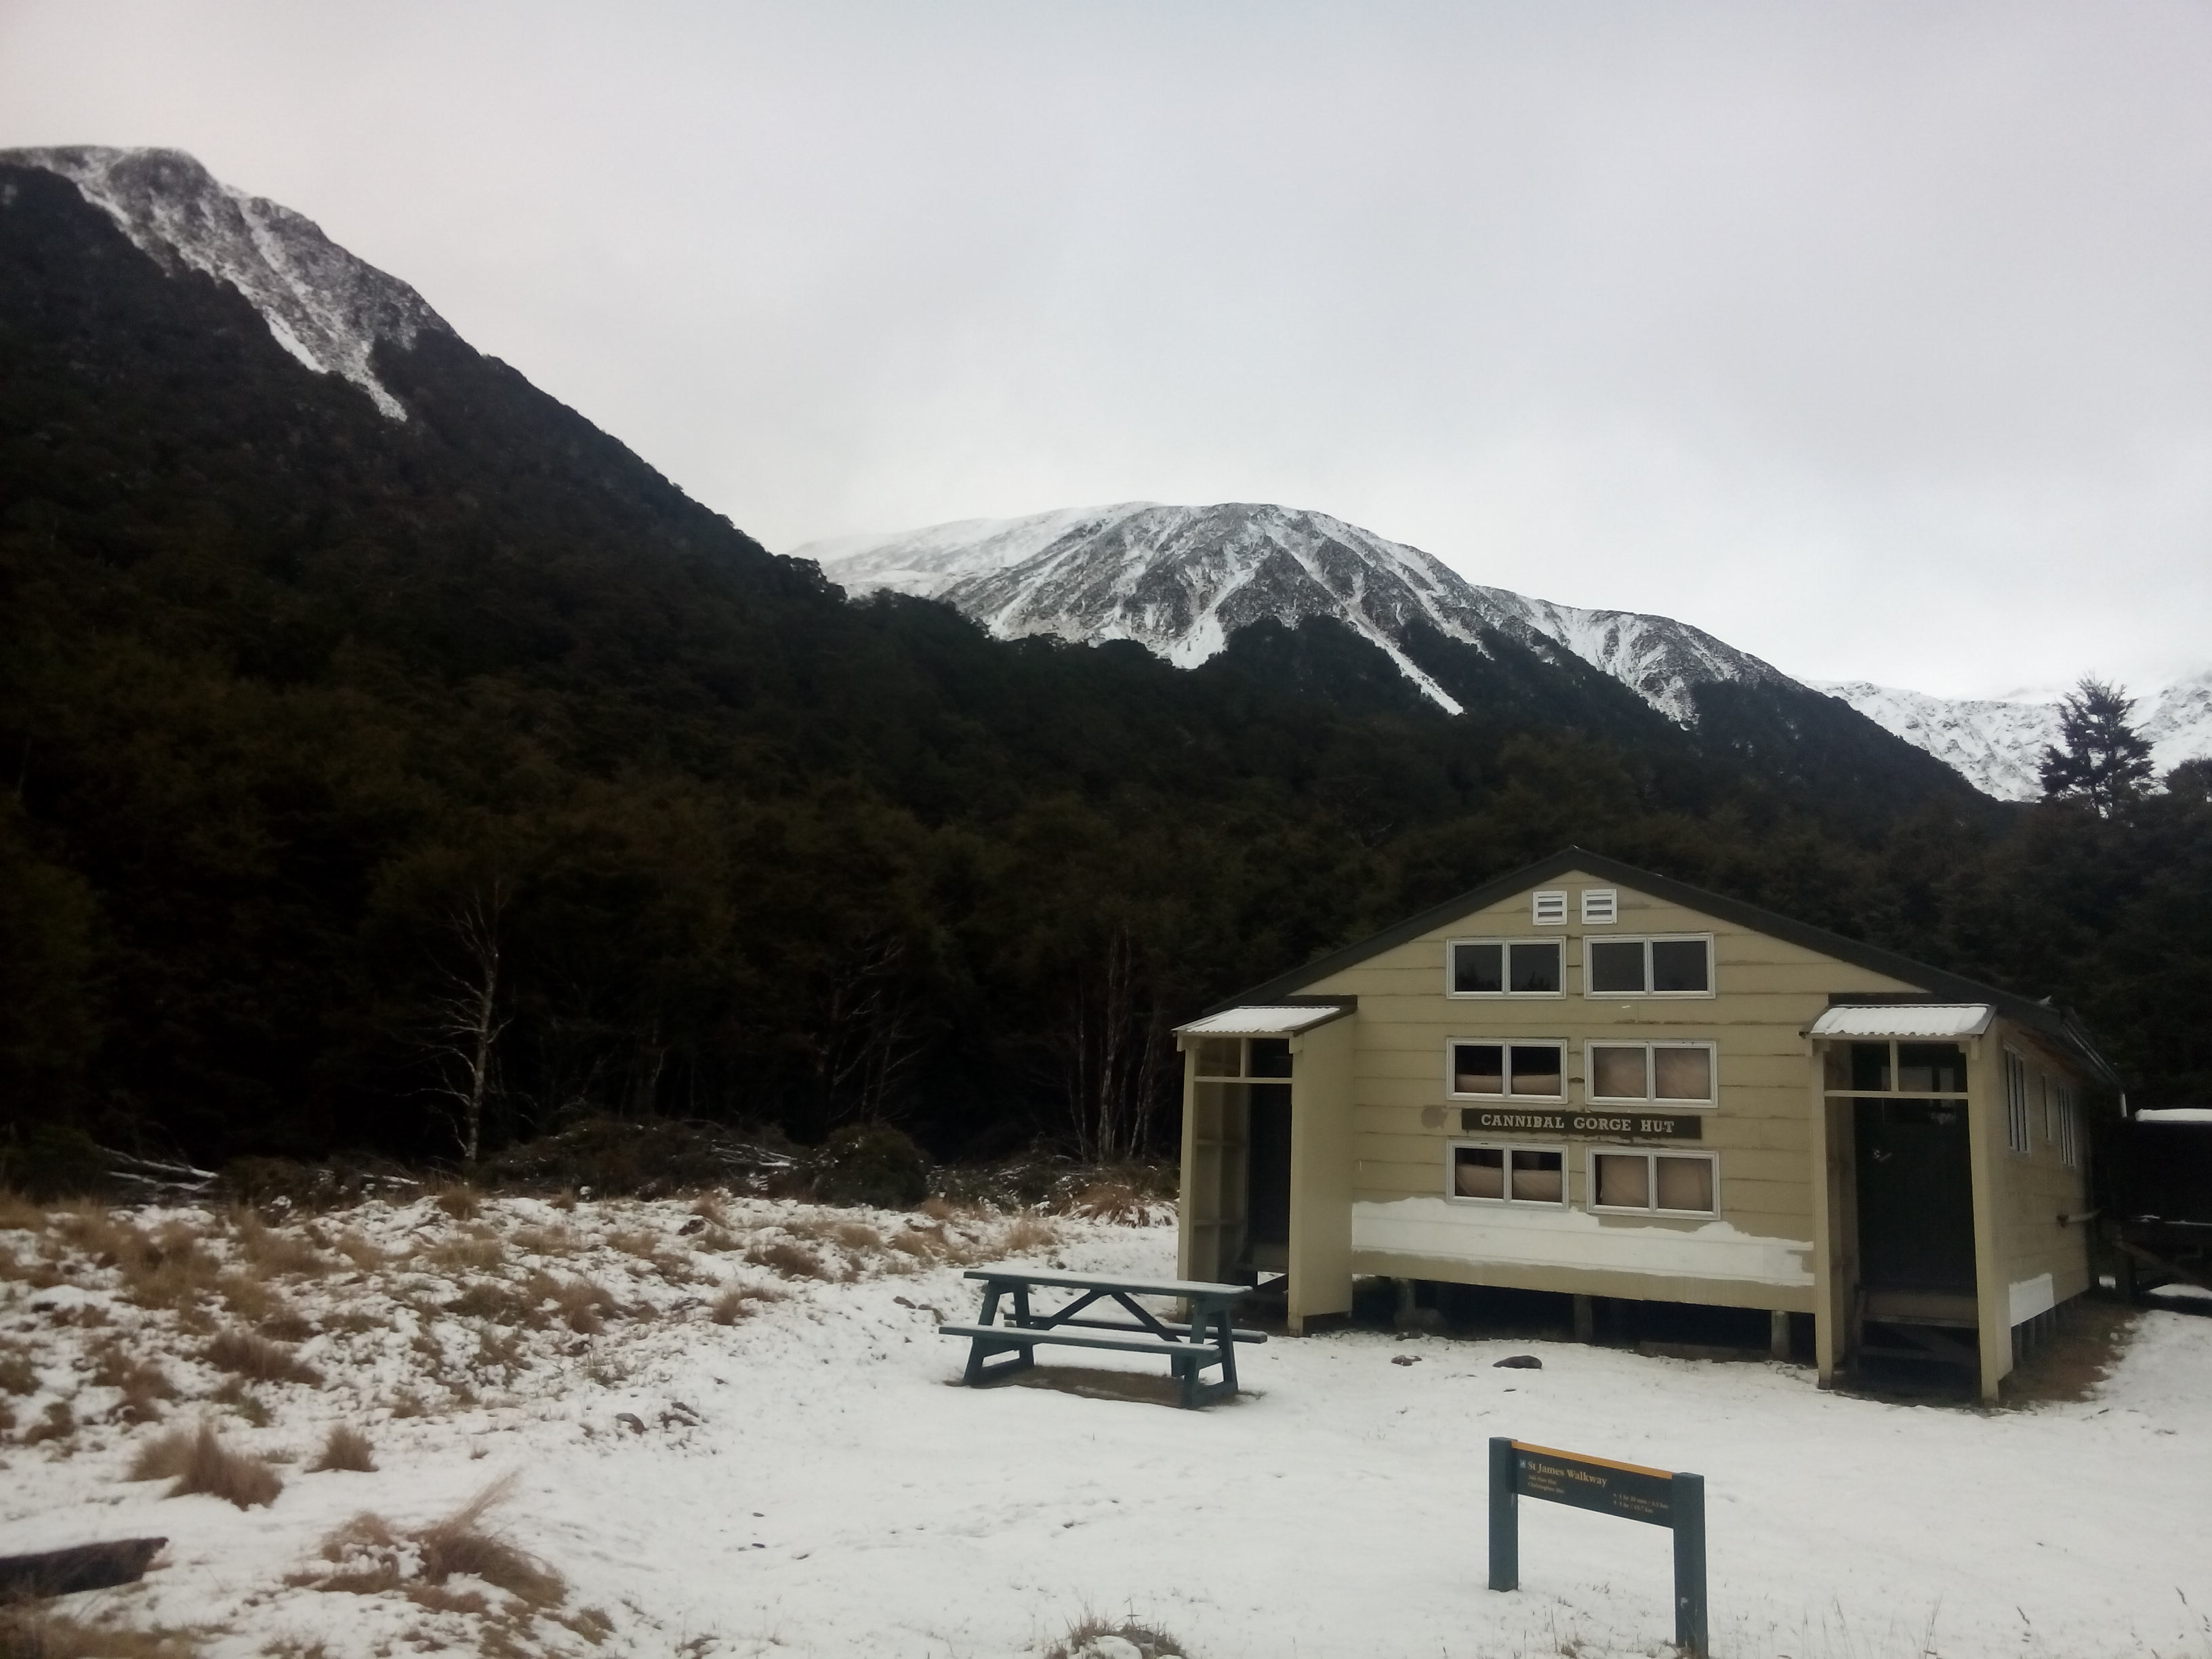
\includegraphics[width=8.5cm]{CannibalGorgeHut15June2017Photo1}
\end{flushleft}
\end{minipage}
\begin{minipage}{.5\linewidth}
\begin{flushright}
    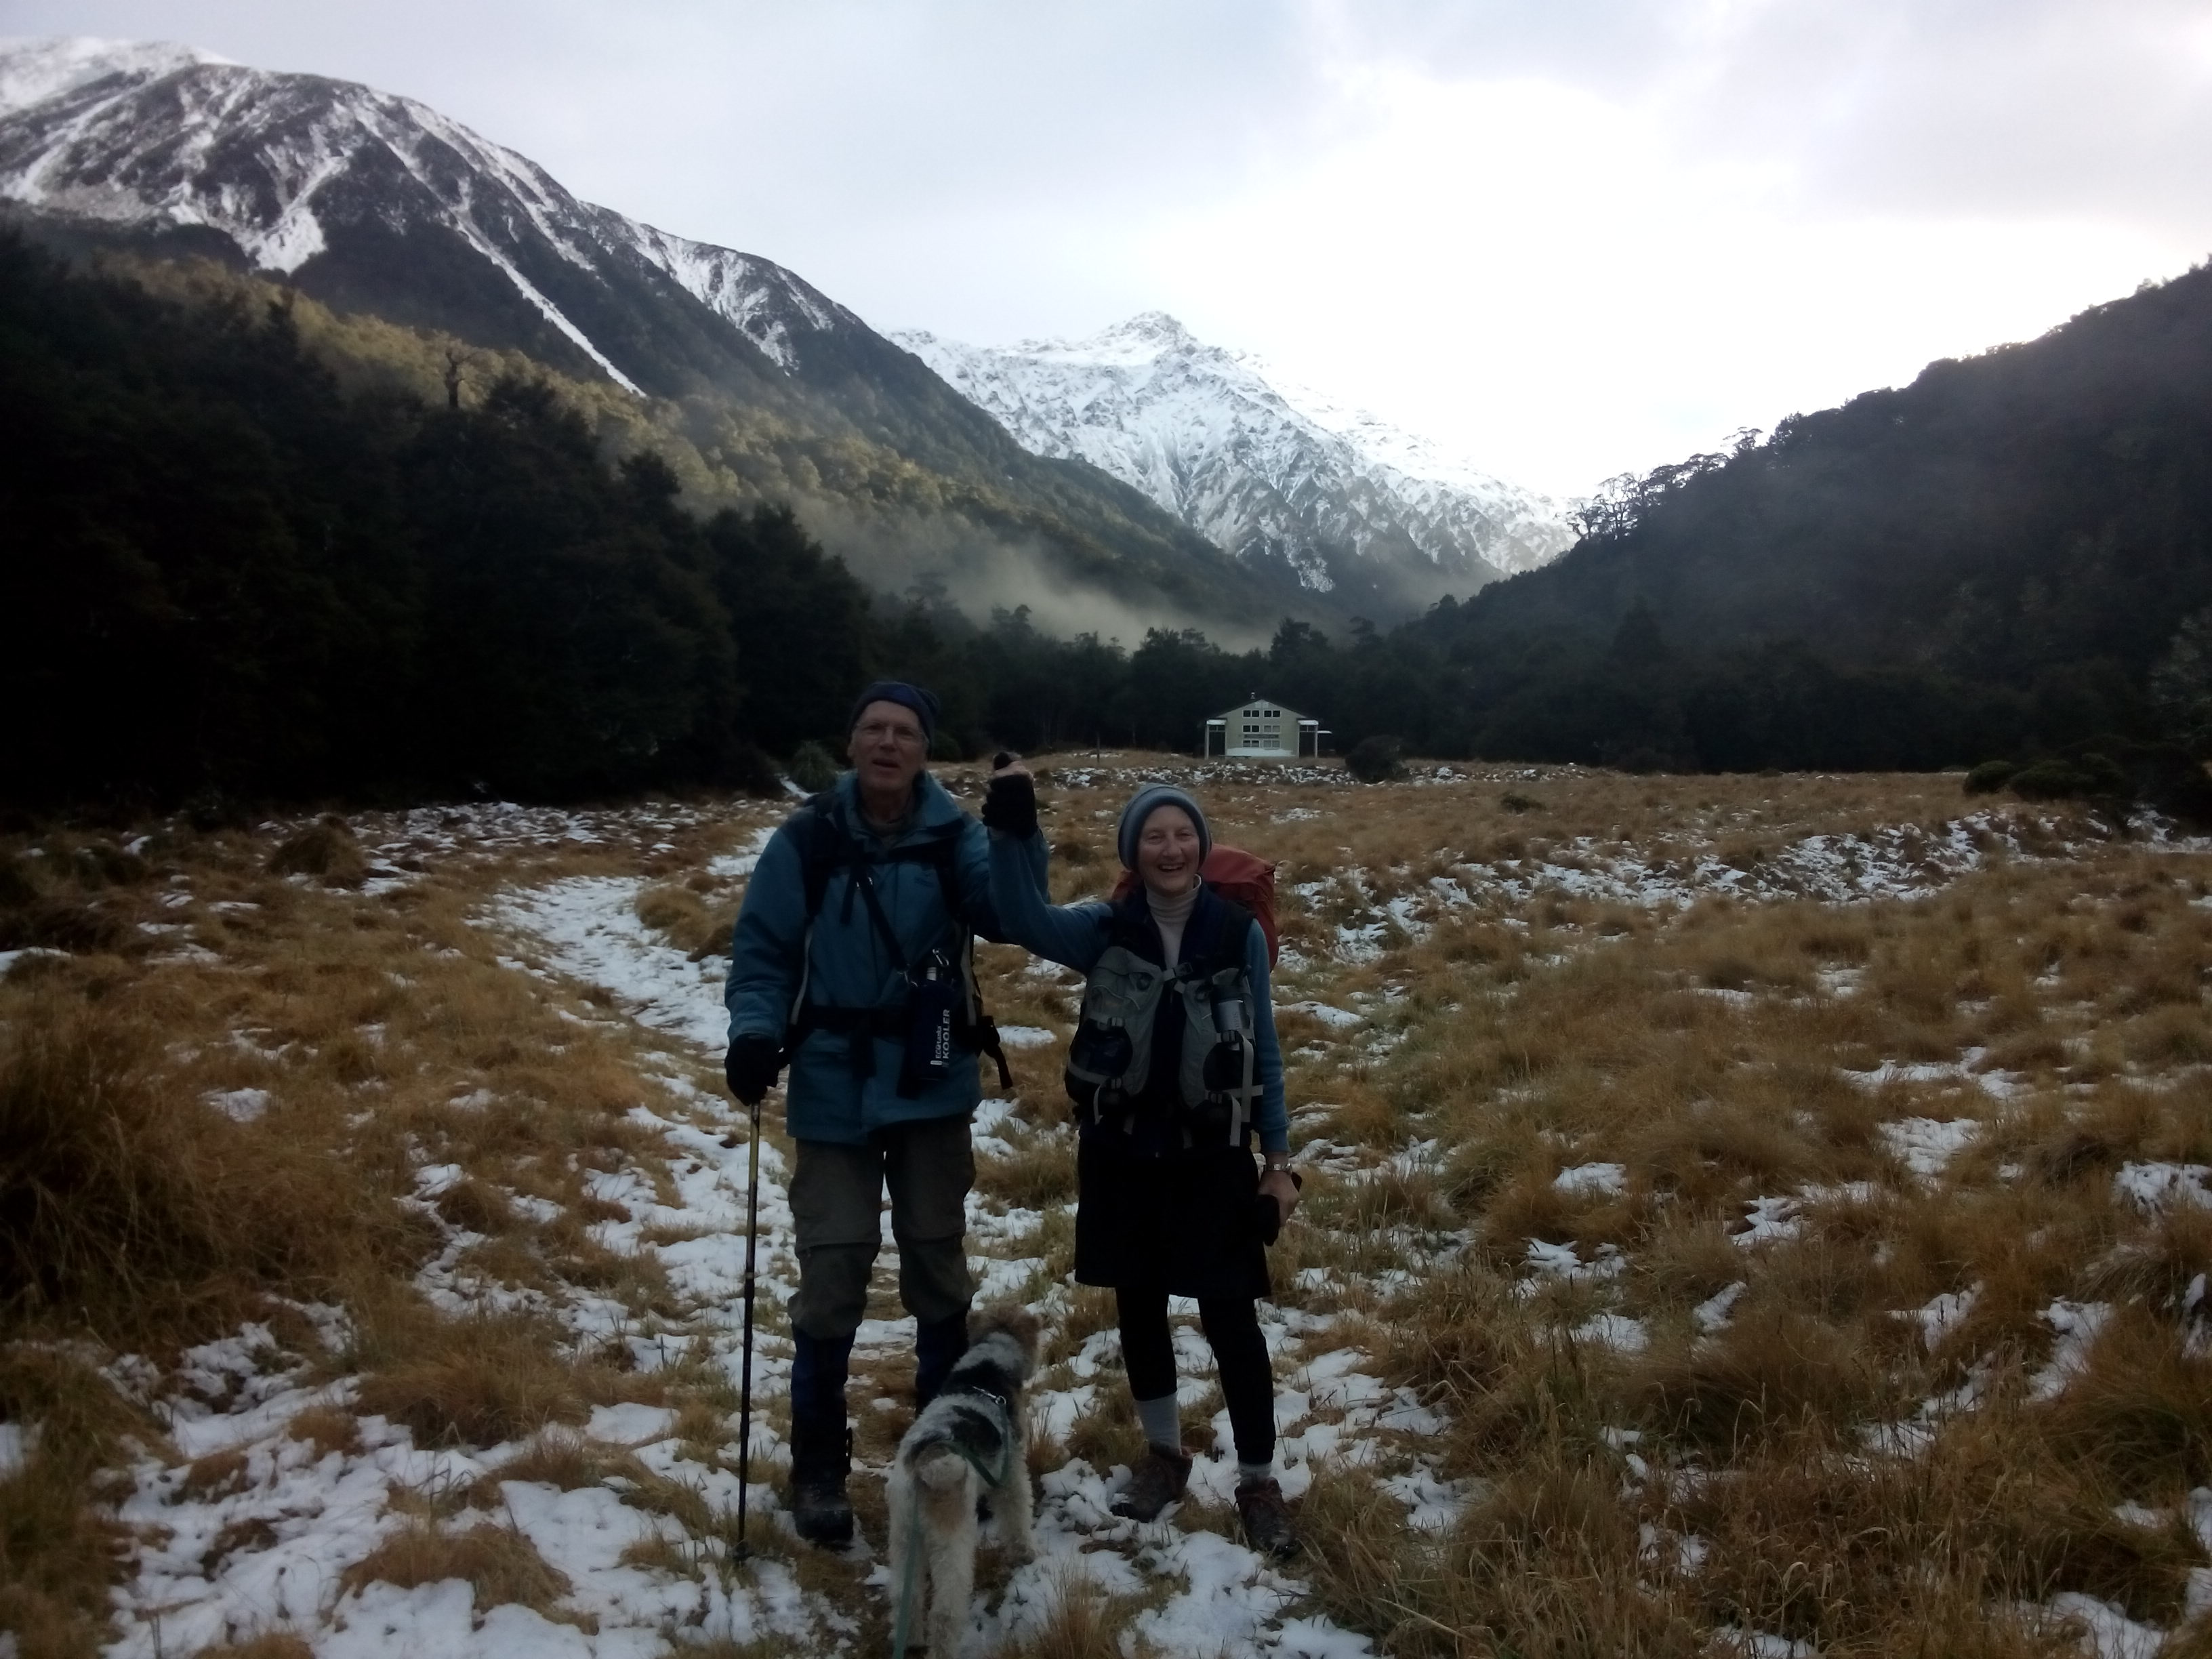
\includegraphics[width=8.5cm]{CannibalGorgeHut15June2017Photo2}
\end{flushright}
\end{minipage}
\end{figure}

Although there were plenty of recently felled trees and firewood rounds, there was little dry wood at the hut.  Thus getting the fire going was an interesting wee challenge, but we succeeded.  As Pierre needed to be warm we burnt quite a bit of coal - and managed to raise the hut temperature to a balmy 6$^o$C from 1$^o$C.  We left the hut stocked with cut wood ready for burning, and split a supply for the wood shed.

The return trip took a little longer than going in.  There was quite a bit of bird life present: robins, tomtits and riflemen.


\begin{flushright}
Pierre, Robyn, Peter and dog
\end{flushright}

\end{document}
